\documentclass[lettersize,journal]{IEEEtran}
\usepackage{amsmath,amsfonts}
\usepackage{algorithmic}
\usepackage{algorithm}
\usepackage{array}
\usepackage[caption=false,font=normalsize,labelfont=sf,textfont=sf]{subfig}
\usepackage{textcomp}
\usepackage{stfloats}
\usepackage{url}
\usepackage{verbatim}
\usepackage{graphicx}
\usepackage{cite}
\hyphenation{op-tical net-works semi-conduc-tor IEEE-Xplore}

\begin{document}

\title{Fuzzy Logic-Driven Adaptive Semantic Communication for the Internet of Vehicles}

\author{
Author~1,
Author~2,
Author~3
\thanks{
This work was supported in part by XXX.
}
\thanks{
The authors are with XXX University/Institute.
}
}

\markboth{IEEE Transactions on Vehicular Technology,~2026}%
{Author \MakeLowercase{\textit{et al.}}: Fuzzy Logic-Driven Adaptive Semantic Communication for the Internet of Vehicles}

% \IEEEpubid{0000--0000/00\$00.00~\copyright~2026 IEEE}

\maketitle

%%%%%%%%%%%%%%%%%%%%%%%%%%%%%%%%%%%%%%%%%%%%%%%%%%%%%%%%%%%%%%%%%%%%%%%%%%%%%%%%
\begin{abstract}

Semantic communication has emerged as a promising solution for efficient data transmission in Internet of Vehicles (IoV) environments. However, conventional semantic communication systems either transmit all data through semantic encoders regardless of channel conditions or rely on direct transmission strategies that fail to adapt to dynamic vehicular environments. In this paper, we propose a Fuzzy Logic-Driven Adaptive Semantic Communication framework for IoV that dynamically selects transmission strategies based on real-time channel quality, distance, and vehicle mobility conditions. The proposed framework integrates fuzzy logic decision-making with adaptive semantic transmission to improve communication quality while reducing unnecessary computational overhead. Experimental results demonstrate that the proposed method significantly improves Peak Signal-to-Noise Ratio (PSNR) and transmission accuracy compared with direct transmission approaches, while consuming fewer computational resources than fully semantic transmission schemes. Extensive evaluations under varying signal-to-noise ratio (SNR), distance, and relative speed conditions validate the effectiveness and robustness of the proposed approach for intelligent vehicular communications.

\end{abstract}

\begin{IEEEkeywords}

Semantic communication, Internet of Vehicles (IoV), fuzzy logic, adaptive transmission, vehicular networks, PSNR, intelligent transportation systems.

\end{IEEEkeywords}

%%%%%%%%%%%%%%%%%%%%%%%%%%%%%%%%%%%%%%%%%%%%%%%%%%%%%%%%%%%%%%%%%%%%%%%%%%%%%%%%
\section{Introduction}

\IEEEPARstart{T}{he} rapid development of intelligent transportation systems and autonomous driving technologies has significantly increased the demand for reliable and efficient vehicular communications. Internet of Vehicles (IoV) applications require ultra-reliable and low-latency communication under highly dynamic wireless environments characterized by rapidly changing channel conditions, vehicle mobility, and interference.

Traditional communication systems based on Shannon theory focus on accurate bit-level transmission, often leading to inefficient resource utilization in bandwidth-constrained vehicular environments. Recently, semantic communication has emerged as a promising paradigm that prioritizes the transmission of semantic information rather than exact bit reconstruction. By leveraging deep learning-based semantic encoders and decoders, semantic communication systems can achieve higher robustness and compression efficiency under noisy channels.

Despite these advantages, existing semantic communication approaches face two major limitations in IoV scenarios:
\begin{itemize}
    \item Always transmitting through semantic models introduces unnecessary computational overhead under favorable channel conditions.
    \item Direct transmission approaches fail to maintain communication quality under severe channel degradation and mobility.
\end{itemize}

To address these challenges, this paper proposes a fuzzy logic-driven adaptive semantic communication framework that dynamically switches between transmission strategies according to channel conditions and vehicular dynamics.

The main contributions of this paper are summarized as follows:
\begin{itemize}
    \item We propose a fuzzy logic-based adaptive transmission framework for semantic communication in IoV environments.
    
    \item We design a dynamic decision-making mechanism that jointly considers SNR, transmission distance, and relative vehicle speed.
    
    \item We develop an adaptive semantic communication architecture that balances communication quality and computational efficiency.
    
    \item We conduct extensive experiments under varying vehicular conditions and demonstrate that the proposed method improves PSNR and transmission accuracy compared with direct transmission methods while reducing computational costs compared with fully semantic transmission schemes.
\end{itemize}

The remainder of this paper is organized as follows. Section II reviews related works. Section III introduces the proposed system model and fuzzy logic framework. Section IV presents the experimental setup. Section V discusses the experimental results and analysis. Finally, Section VI concludes the paper and outlines future research directions.

%%%%%%%%%%%%%%%%%%%%%%%%%%%%%%%%%%%%%%%%%%%%%%%%%%%%%%%%%%%%%%%%%%%%%%%%%%%%%%%%
\section{Related Work}

\subsection{Semantic Communication Systems}

\begin{itemize}
    \item Overview of semantic communication theory
    \item Deep learning-based semantic encoding and decoding
    \item Joint source-channel coding (JSCC)
    \item Semantic communication for wireless networks
\end{itemize}

\subsection{Semantic Communication in Vehicular Networks}

\begin{itemize}
    \item Challenges in IoV communications
    \item Dynamic channel characteristics in vehicular environments
    \item Existing semantic communication approaches for IoV
\end{itemize}

\subsection{Adaptive Transmission Techniques}

\begin{itemize}
    \item Adaptive modulation and coding
    \item SNR-aware transmission strategies
    \item Resource allocation in vehicular communications
\end{itemize}

\subsection{Fuzzy Logic in Wireless Communications}

\begin{itemize}
    \item Fundamentals of fuzzy logic systems
    \item Fuzzy decision-making for network optimization
    \item Applications in intelligent vehicular systems
\end{itemize}

%%%%%%%%%%%%%%%%%%%%%%%%%%%%%%%%%%%%%%%%%%%%%%%%%%%%%%%%%%%%%%%%%%%%%%%%%%%%%%%%
\section{System Model and Proposed Method}

\subsection{Overall System Architecture}

\begin{itemize}
    \item Transmitter architecture
    \item Receiver architecture
    \item Semantic encoder-decoder pipeline
    \item Wireless channel model
\end{itemize}

\subsection{Vehicular Communication Scenario}

\begin{itemize}
    \item IoV network assumptions
    \item Mobility model
    \item Distance and relative speed considerations
\end{itemize}

\subsection{Adaptive Semantic Communication Framework}

\begin{itemize}
    \item Direct transmission mode
    \item Semantic transmission mode
    \item Hybrid adaptive switching mechanism
\end{itemize}

\subsection{Fuzzy Logic Decision System}

\subsubsection{Input Variables}

\begin{itemize}
    \item Signal-to-Noise Ratio (SNR)
    \item Vehicle distance
    \item Relative speed
\end{itemize}

\subsubsection{Membership Functions}

\begin{itemize}
    \item Low/Medium/High SNR
    \item Near/Mid/Far distance
    \item Slow/Moderate/Fast relative speed
\end{itemize}

\subsubsection{Fuzzy Rules}

Example rules:
\begin{itemize}
    \item IF SNR is High AND Distance is Near THEN Direct Transmission
    \item IF SNR is Low OR Distance is Far THEN Semantic Transmission
    \item IF Relative Speed is High THEN Adaptive Semantic Mode
\end{itemize}

\subsubsection{Defuzzification Strategy}

\begin{itemize}
    \item Decision score computation
    \item Final transmission mode selection
\end{itemize}

\subsection{Complexity Analysis}

\begin{itemize}
    \item Computational complexity
    \item Resource consumption analysis
    \item Comparison with fully semantic transmission
\end{itemize}

%%%%%%%%%%%%%%%%%%%%%%%%%%%%%%%%%%%%%%%%%%%%%%%%%%%%%%%%%%%%%%%%%%%%%%%%%%%%%%%%
\section{Experimental Setup}

\subsection{Dataset Description}

\begin{itemize}
    \item CIFAR-10 dataset
    \item Data preprocessing
    \item Training-validation split
\end{itemize}

\subsection{Neural Network Architecture}

\begin{itemize}
    \item Semantic encoder architecture
    \item Semantic decoder architecture
    \item Classifier model
\end{itemize}

\subsection{Wireless Channel Configuration}

\begin{itemize}
    \item AWGN channel
    \item Rayleigh fading model (optional)
    \item SNR range settings
\end{itemize}

\subsection{Evaluation Metrics}

\begin{itemize}
    \item Peak Signal-to-Noise Ratio (PSNR)
    \item Classification accuracy
    \item Computational complexity
    \item Resource utilization
    \item Transmission latency
\end{itemize}

\subsection{Baseline Methods}

\begin{itemize}
    \item Direct transmission
    \item Fully semantic transmission
    \item Fixed-SNR semantic transmission
    \item Proposed fuzzy logic adaptive method
\end{itemize}

%%%%%%%%%%%%%%%%%%%%%%%%%%%%%%%%%%%%%%%%%%%%%%%%%%%%%%%%%%%%%%%%%%%%%%%%%%%%%%%%
\section{Experimental Results and Discussion}

\subsection{PSNR Performance Analysis}

\begin{itemize}
    \item PSNR versus SNR
    \item PSNR versus transmission distance
    \item PSNR versus relative vehicle speed
\end{itemize}

\begin{figure*}[!t]
\centering
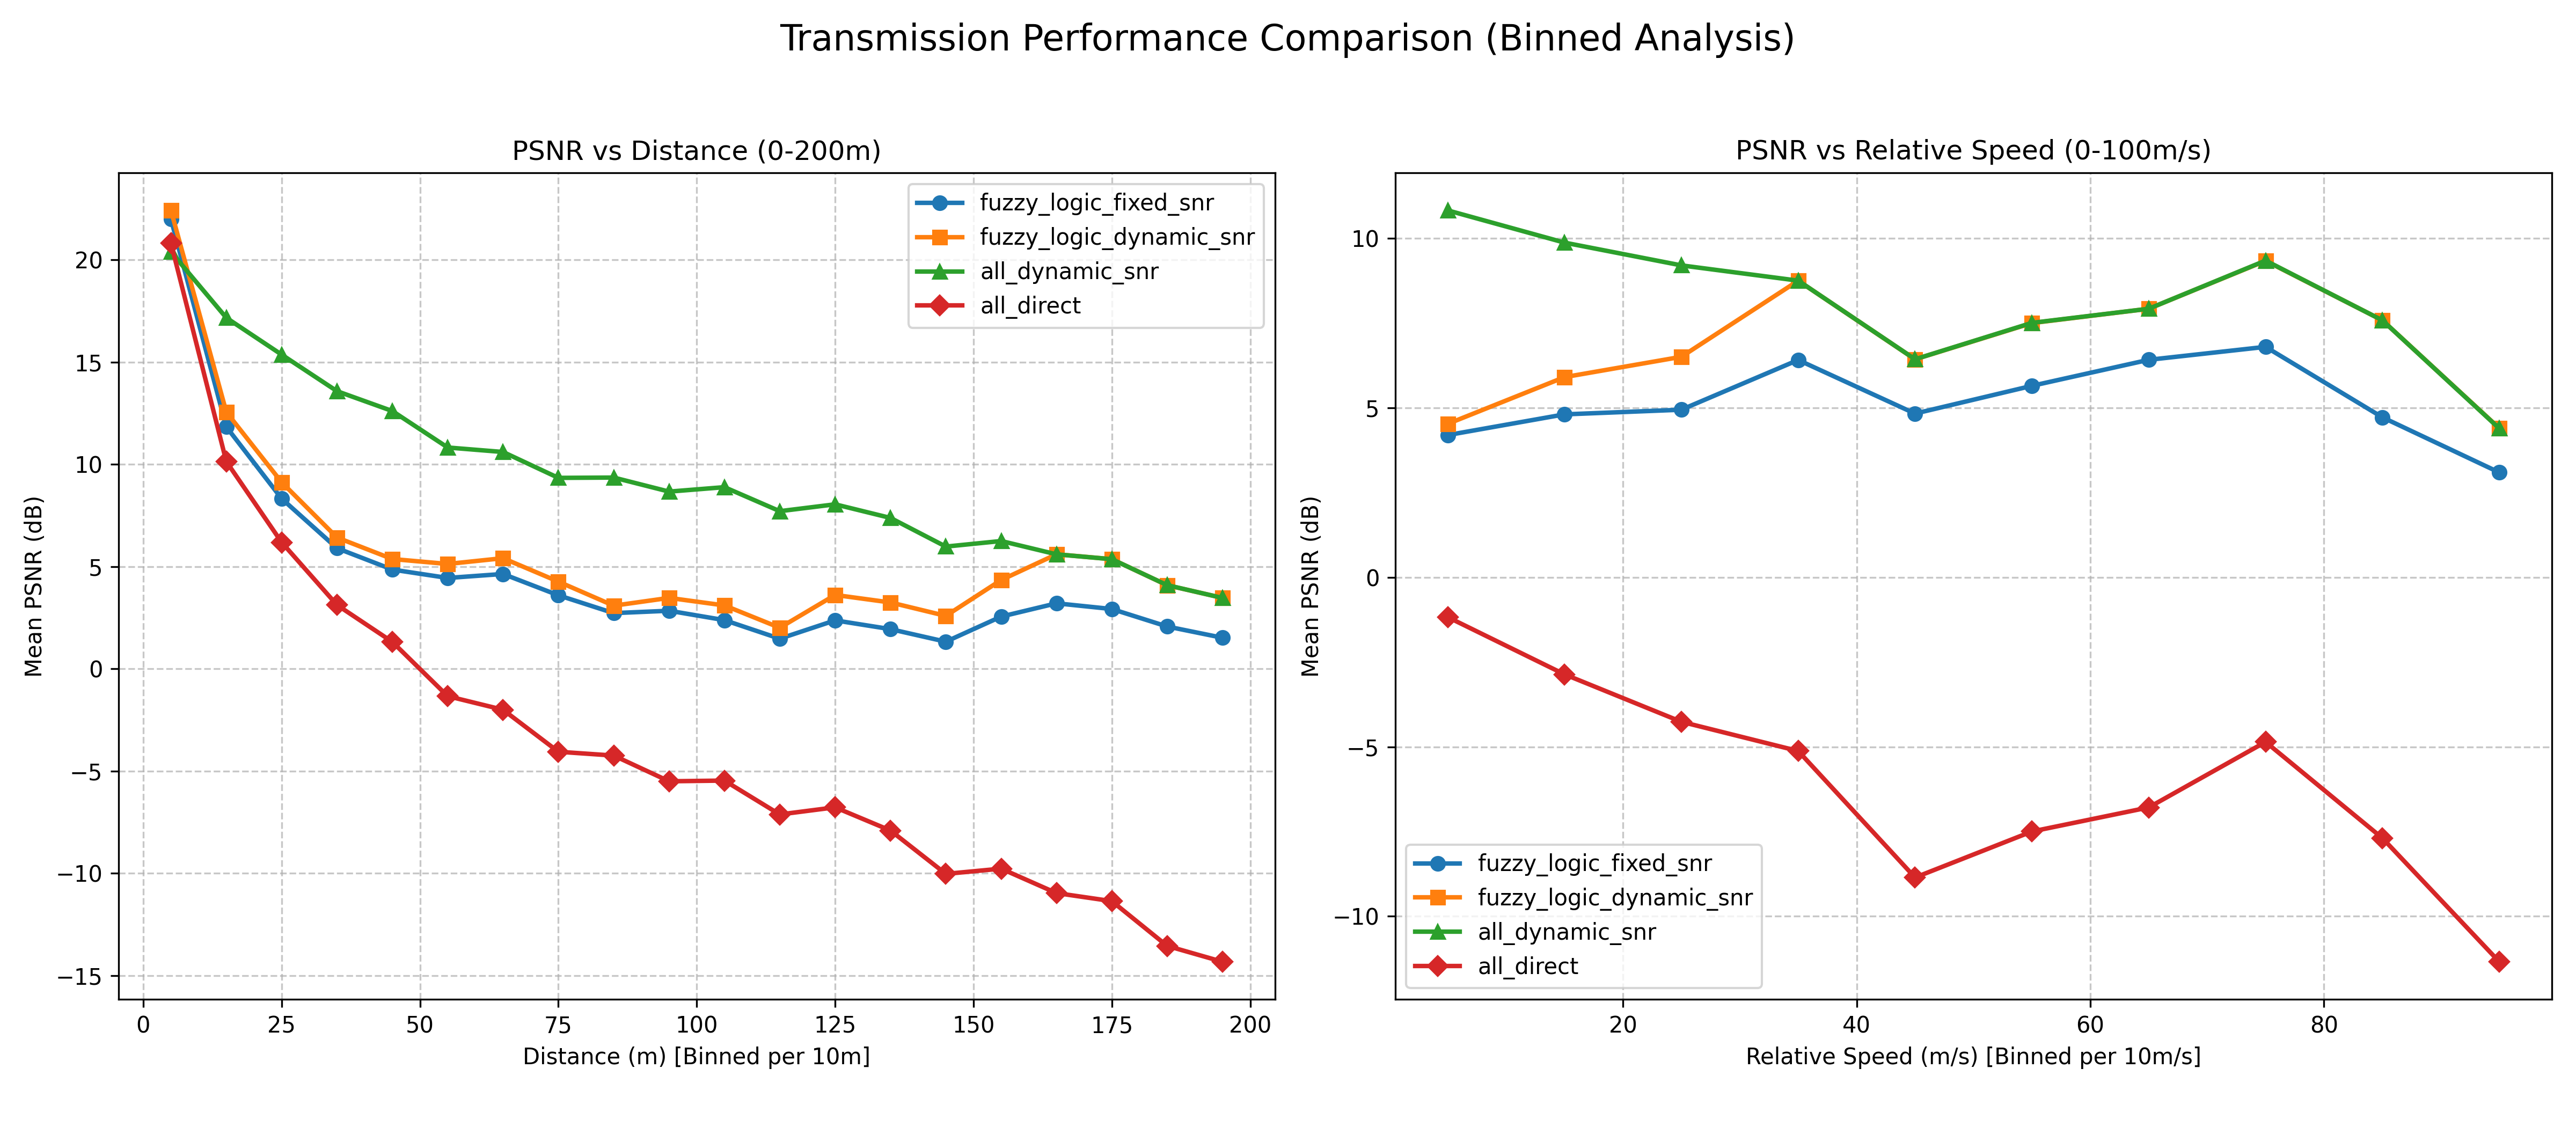
\includegraphics[width=0.95\textwidth]{transmission_comparison_binned_exp_20260513.png}
\caption{
Transmission performance comparison under varying distance and relative speed conditions. The proposed fuzzy logic-driven adaptive semantic communication method achieves higher PSNR performance than direct transmission while maintaining lower computational overhead than fully semantic transmission.
}
\label{fig:performance_comparison}
\end{figure*}

\subsection{Transmission Accuracy Analysis}

\begin{itemize}
    \item Classification accuracy comparison
    \item Robustness under noisy channels
    \item Performance under mobility
\end{itemize}

\subsection{Computational Resource Analysis}

\begin{itemize}
    \item Encoder activation frequency
    \item Computational savings
    \item Trade-off between quality and complexity
\end{itemize}

\subsection{Adaptive Decision Behavior}

\begin{itemize}
    \item Fuzzy decision visualization
    \item Switching behavior analysis
    \item Interpretation of adaptive transmission choices
\end{itemize}

\subsection{Discussion}

\begin{itemize}
    \item Advantages of fuzzy logic adaptation
    \item Impact on IoV reliability
    \item Scalability considerations
    \item Limitations of the current framework
\end{itemize}

%%%%%%%%%%%%%%%%%%%%%%%%%%%%%%%%%%%%%%%%%%%%%%%%%%%%%%%%%%%%%%%%%%%%%%%%%%%%%%%%
\section{Conclusion and Future Work}

This paper proposed a fuzzy logic-driven adaptive semantic communication framework for Internet of Vehicles environments. By dynamically selecting transmission strategies according to channel conditions and vehicular dynamics, the proposed approach improves transmission quality while reducing unnecessary computational overhead. Experimental results demonstrated superior PSNR and accuracy performance compared with direct transmission methods and lower resource consumption than fully semantic communication schemes.

Future work will focus on:
\begin{itemize}
    \item Real-world vehicular deployment
    \item Multi-user semantic communication
    \item Reinforcement learning-enhanced adaptive control
    \item Edge-assisted semantic communication
    \item Integration with 6G vehicular networks
\end{itemize}

%%%%%%%%%%%%%%%%%%%%%%%%%%%%%%%%%%%%%%%%%%%%%%%%%%%%%%%%%%%%%%%%%%%%%%%%%%%%%%%%
\section*{Acknowledgment}

The authors would like to thank XXX for supporting this research.

%%%%%%%%%%%%%%%%%%%%%%%%%%%%%%%%%%%%%%%%%%%%%%%%%%%%%%%%%%%%%%%%%%%%%%%%%%%%%%%%
\bibliographystyle{IEEEtran}
\bibliography{references}

\end{document}